\chapter{Sprint 2 : Parcours de soins et traçabilité}\label{chap5}

\section{Introduction}

Le deuxième sprint couvre le parcours clinique : consultation des médecins et des patients, gestion des rendez-vous et des dossiers médicaux, demande et suivi d'un épisode de traitement. Il introduit également la vérification d'intégrité consultable depuis l'interface patient et médecin.

\section{Objectifs du sprint}

\begin{itemize}
    \item Permettre au patient de demander un traitement et d'abandonner un épisode en cours.
    \item Permettre au médecin d'activer ou de clôturer un épisode.
    \item Gérer les phases et les événements cliniques d'un épisode.
    \item Afficher la timeline de suivi et l'état de vérification des blocs.
    \item Fournir une interface de consultation des ressources cliniques.
\end{itemize}

\section{Contrôle d'accès au parcours de soins}

La Figure \ref{fig:access_seq} illustre le filtrage des données. Le patient demande un traitement, le médecin consulte la timeline de l'épisode, et le backend applique le filtrage selon le rôle. Lorsque l'épisode n'appartient pas à l'utilisateur, la réponse est un \texttt{403 Forbidden} et un événement \texttt{denied} est écrit dans le journal d'audit.

\begin{figure}[H]
\centering
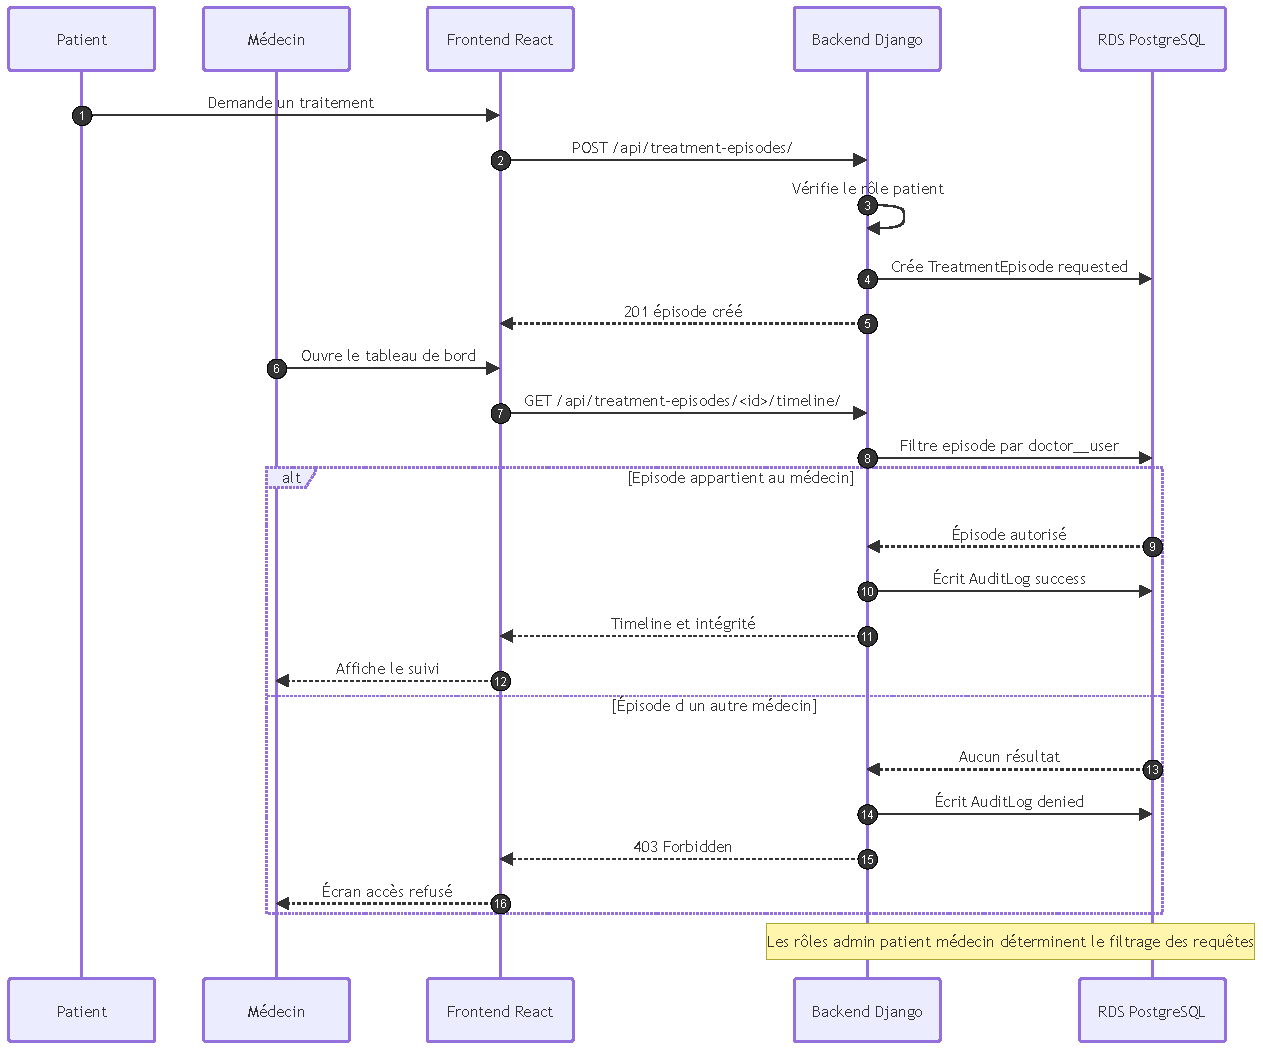
\includegraphics[width=\textwidth]{07-controle-acces-sequence.pdf}
\caption{Séquence de contrôle d'accès à un épisode}
\label{fig:access_seq}
\end{figure}

\section{Cycle de vie d'un traitement}

La Figure \ref{fig:states} décrit les états d'un épisode de traitement et ceux d'une phase. Un épisode passe de \textit{demandé} à \textit{actif} sur action du médecin, puis à \textit{terminé} ou \textit{abandonné}. Une phase peut être \textit{en attente}, \textit{active}, \textit{terminée}, \textit{échouée} ou \textit{ignorée}.

\begin{figure}[H]
\centering
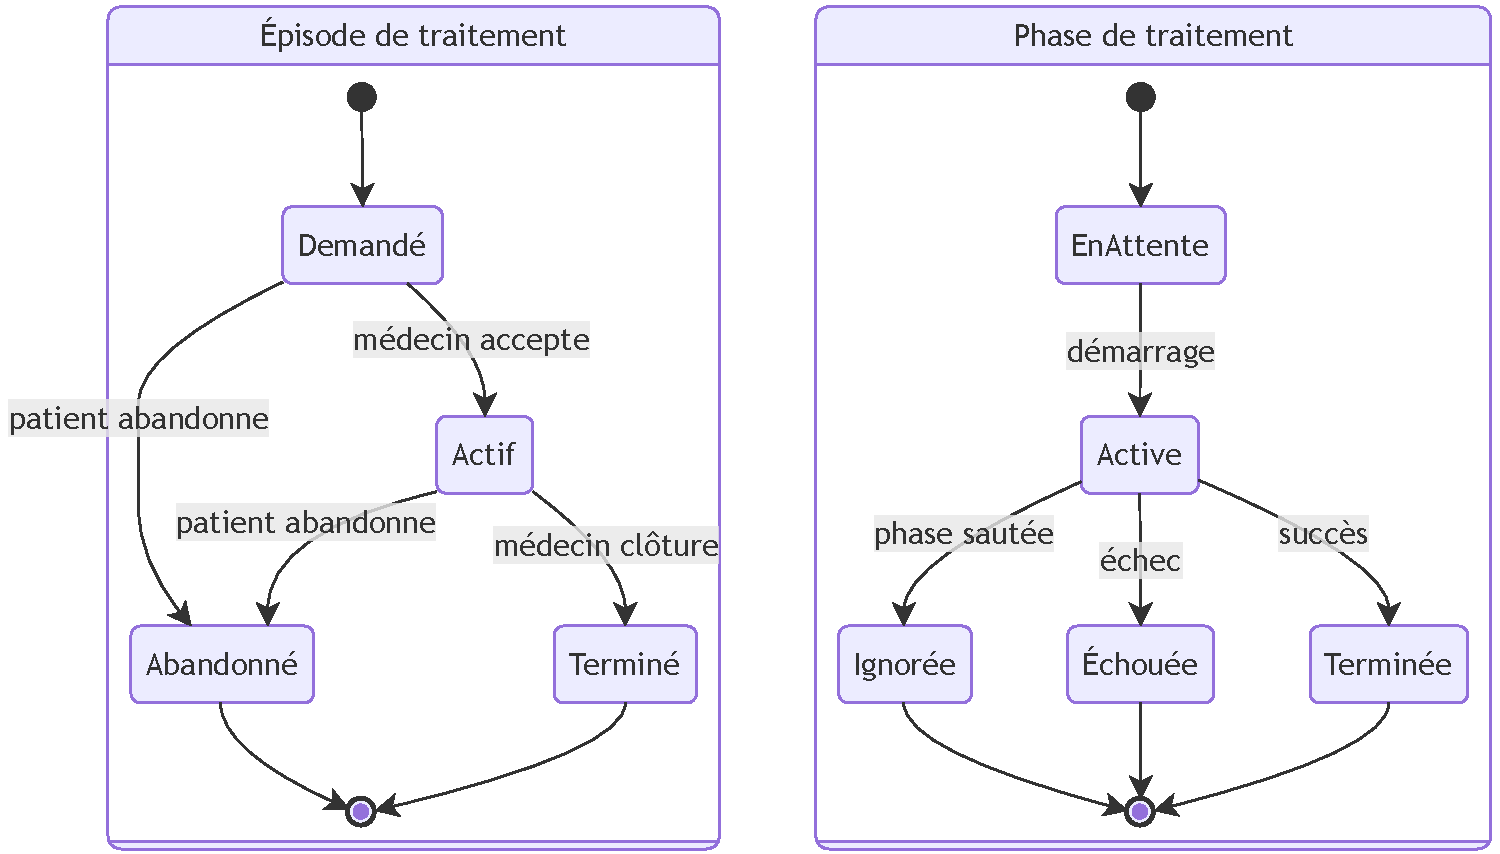
\includegraphics[width=\textwidth]{08-cycle-traitement-etats.pdf}
\caption{Diagrammes d'états du traitement}
\label{fig:states}
\end{figure}

\section{Réalisation --- Espace patient}

La Figure \ref{fig:patient_dash} présente l'espace patient avec la liste des traitements et la demande de suivi. La Figure \ref{fig:integrity} montre le panneau de détails d'intégrité, où le patient peut lire les hashs de blocs, les racines Merkle et les transactions d'ancrage.

\begin{figure}[H]
\centering
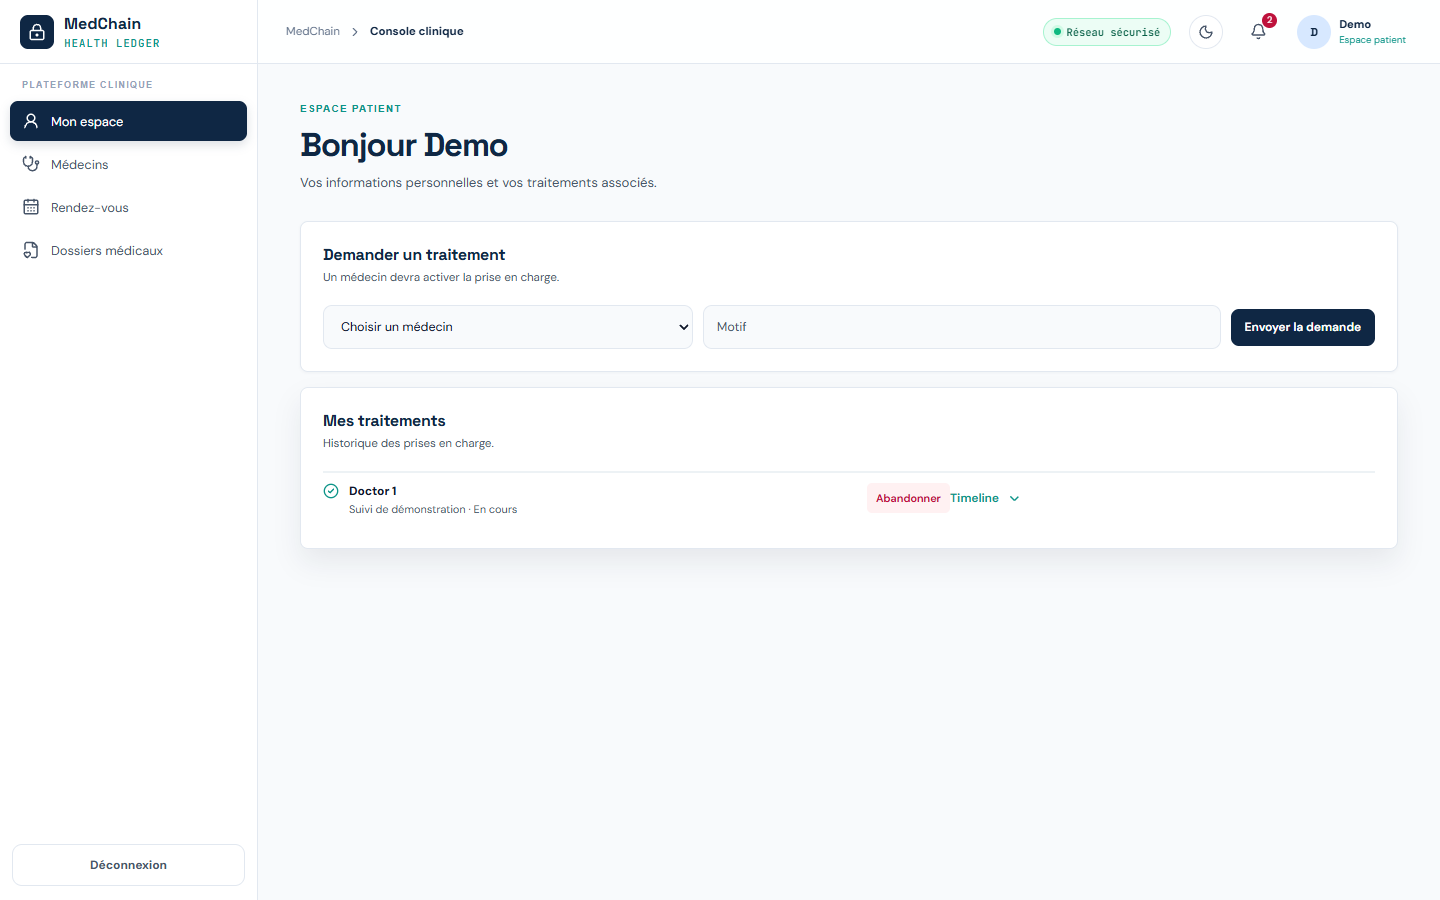
\includegraphics[width=\textwidth]{S04-espace-patient.png}
\caption{Tableau de bord patient}
\label{fig:patient_dash}
\end{figure}

\begin{figure}[H]
\centering
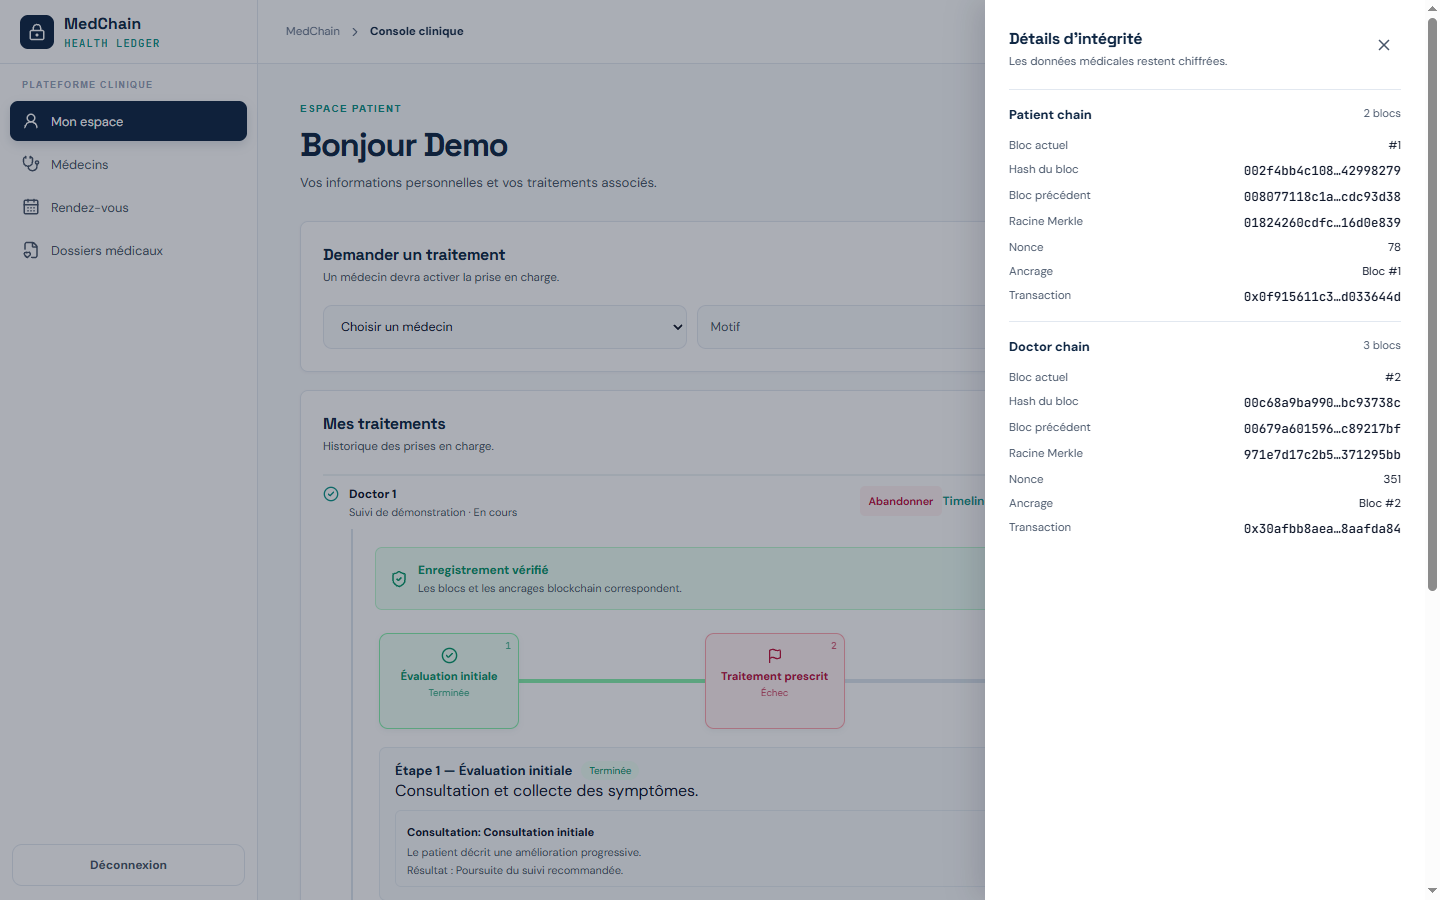
\includegraphics[width=\textwidth]{S05-details-integrite.png}
\caption{Détails d'intégrité des chaînes}
\label{fig:integrity}
\end{figure}

Les Figures \ref{fig:doctors}, \ref{fig:appointments}, \ref{fig:appointment_form} et \ref{fig:records} illustrent la gestion des ressources cliniques.

\begin{figure}[H]
\centering
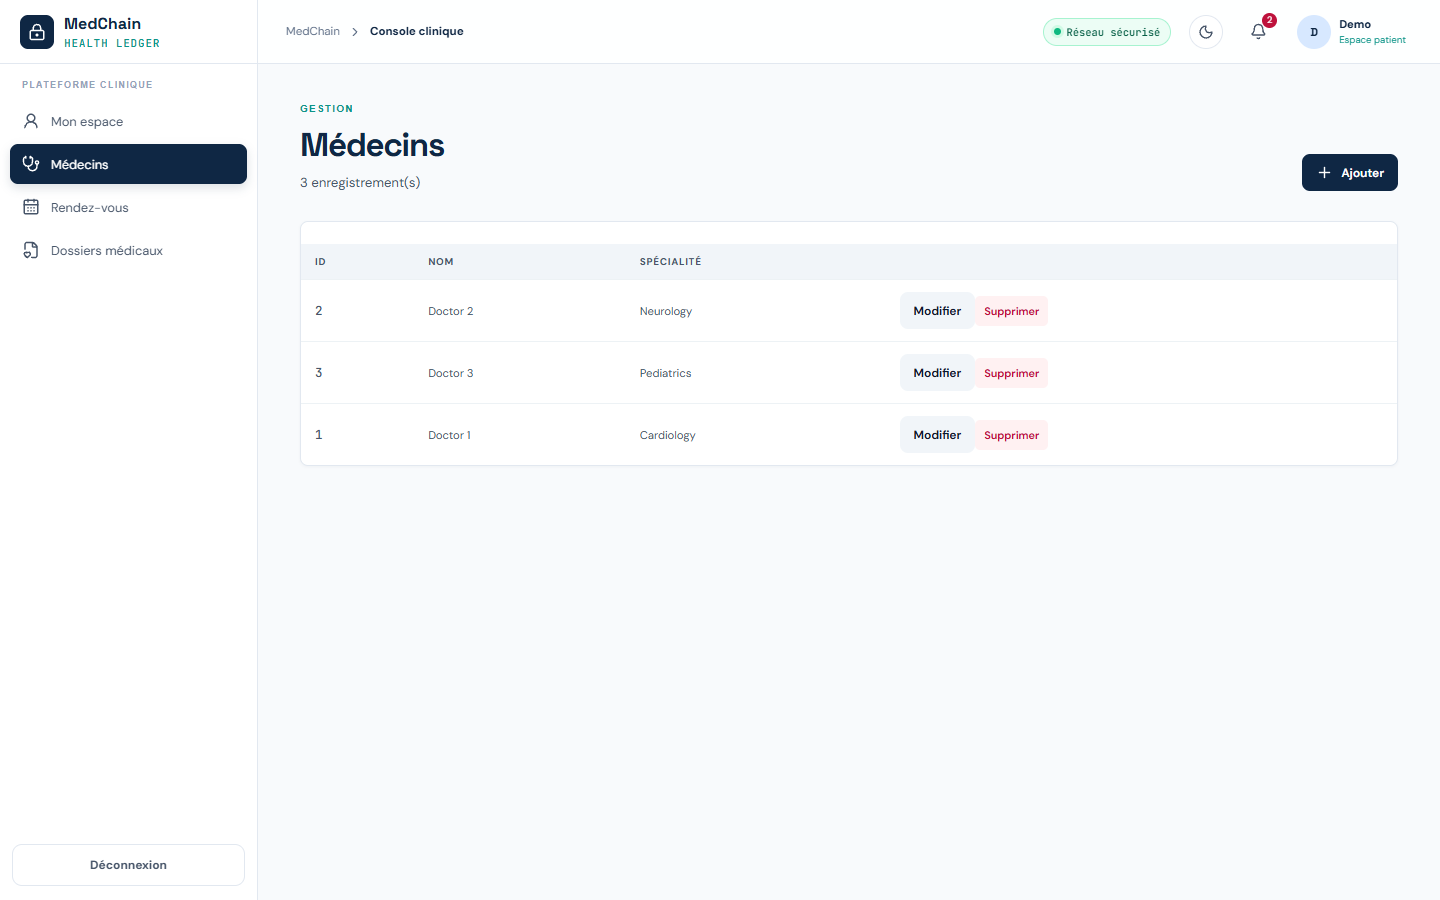
\includegraphics[width=\textwidth]{S06-liste-medecins.png}
\caption{Liste des médecins}
\label{fig:doctors}
\end{figure}

\begin{figure}[H]
\centering
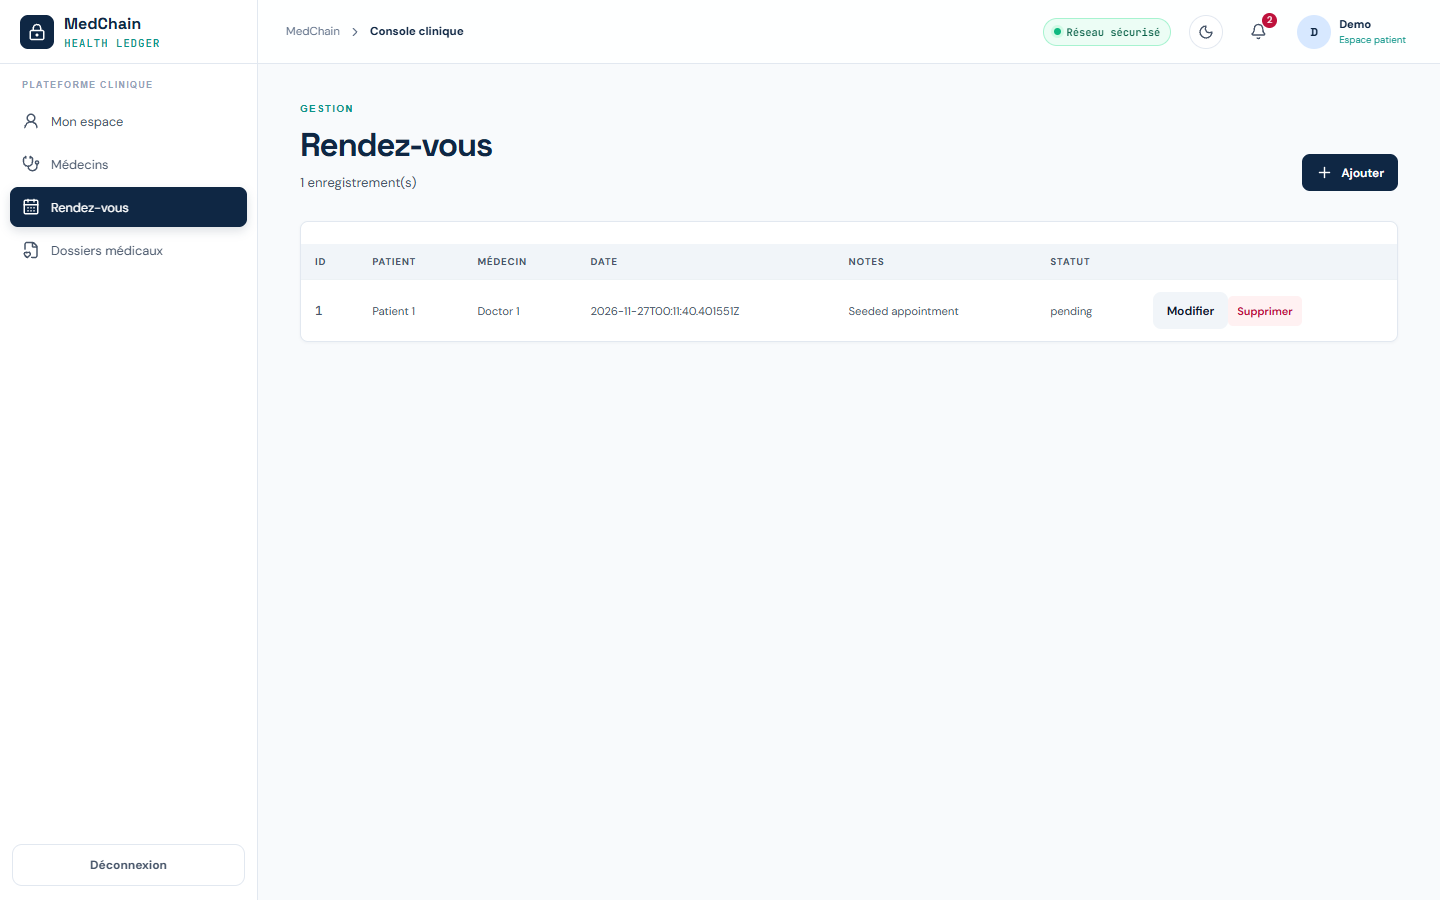
\includegraphics[width=\textwidth]{S07-liste-rendezvous.png}
\caption{Liste des rendez-vous}
\label{fig:appointments}
\end{figure}

\begin{figure}[H]
\centering
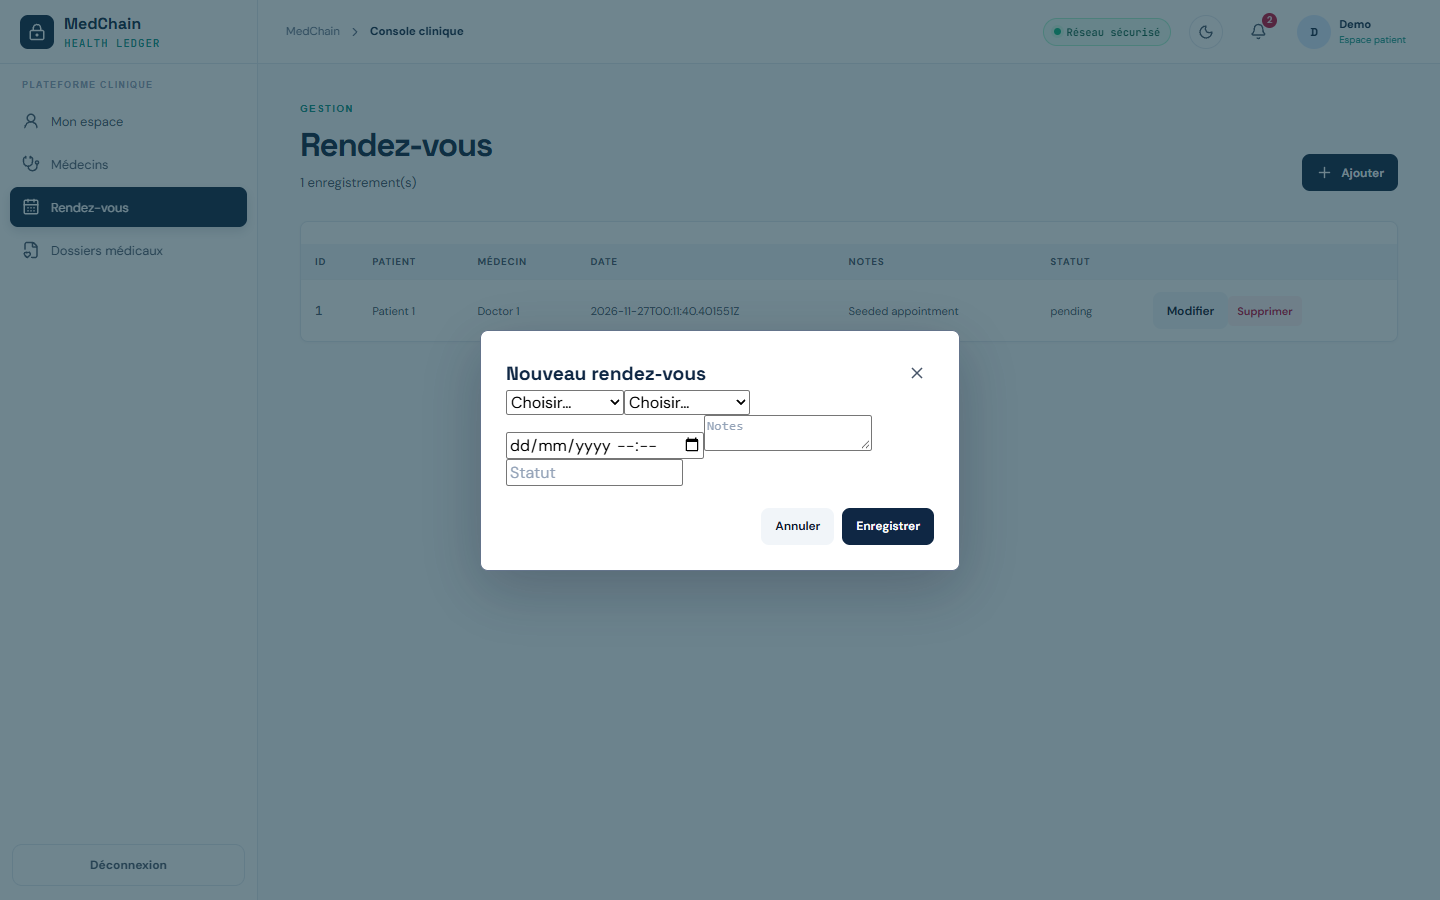
\includegraphics[width=\textwidth]{S08-creation-rendezvous.png}
\caption{Formulaire de création d'un rendez-vous}
\label{fig:appointment_form}
\end{figure}

\begin{figure}[H]
\centering
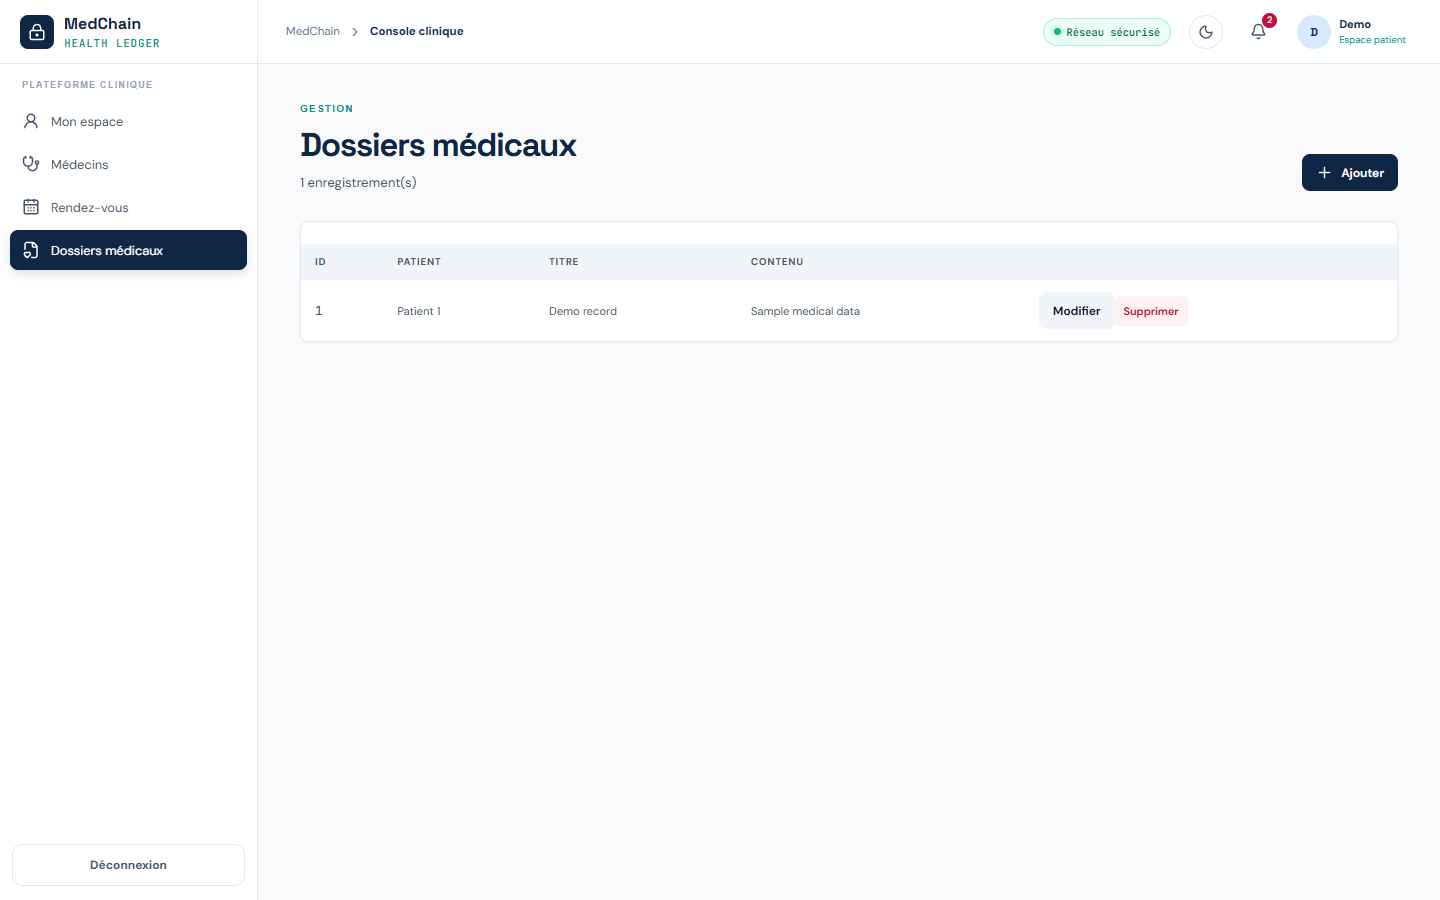
\includegraphics[width=\textwidth]{S09-liste-dossiers.png}
\caption{Liste des dossiers médicaux}
\label{fig:records}
\end{figure}

\section{Réalisation --- Espace médecin}

La Figure \ref{fig:doctor_dash} montre l'espace médecin et la Figure \ref{fig:patients_list} la liste des patients. La Figure \ref{fig:event_form} détaille la timeline d'un épisode et le formulaire d'ajout d'un événement clinique.

\begin{figure}[H]
\centering
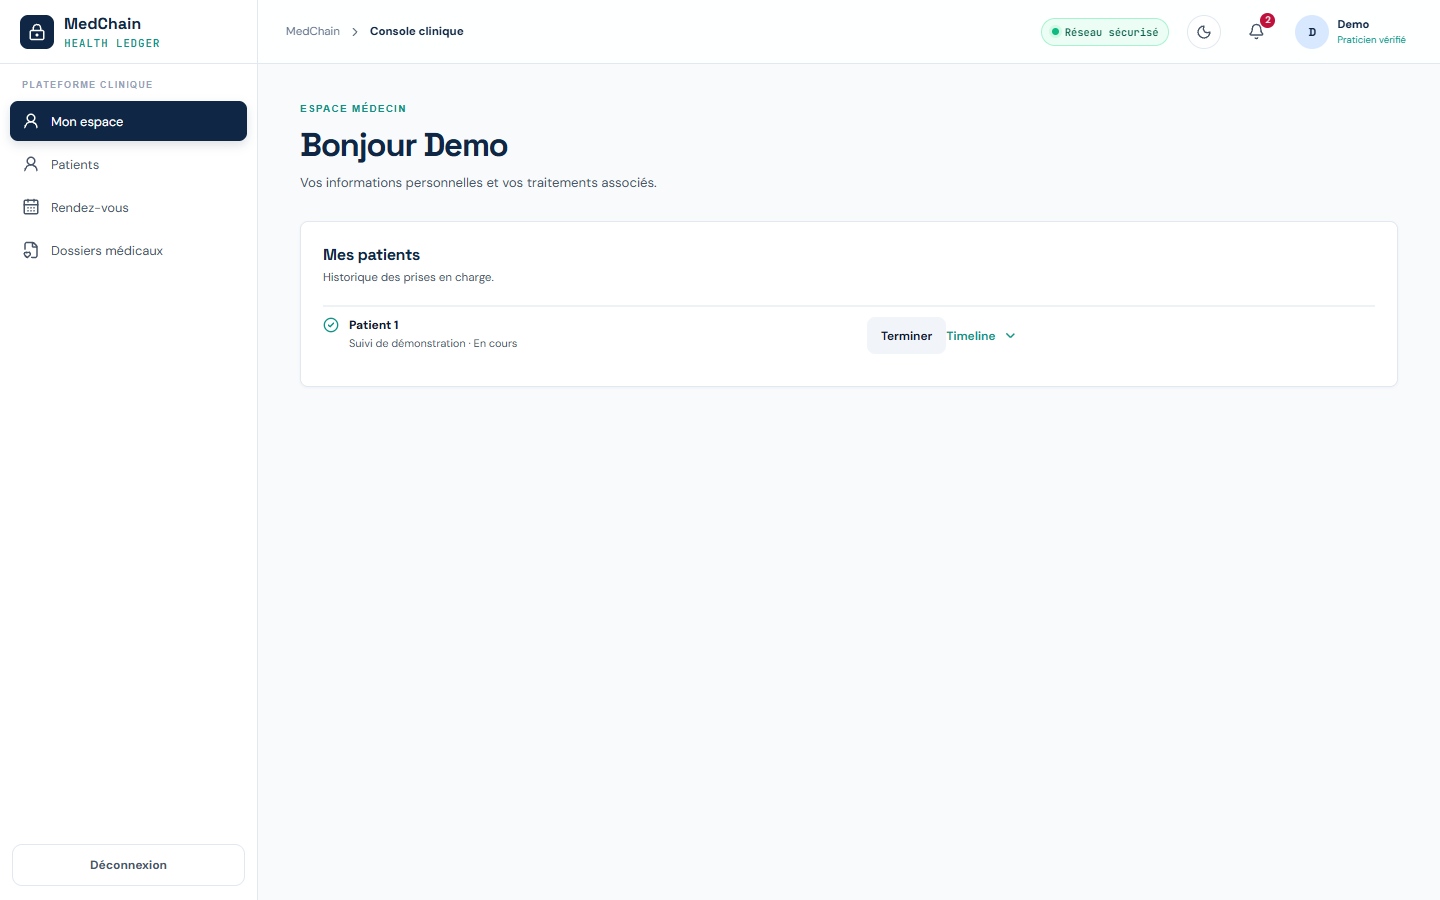
\includegraphics[width=\textwidth]{S11-espace-medecin.png}
\caption{Tableau de bord médecin}
\label{fig:doctor_dash}
\end{figure}

\begin{figure}[H]
\centering
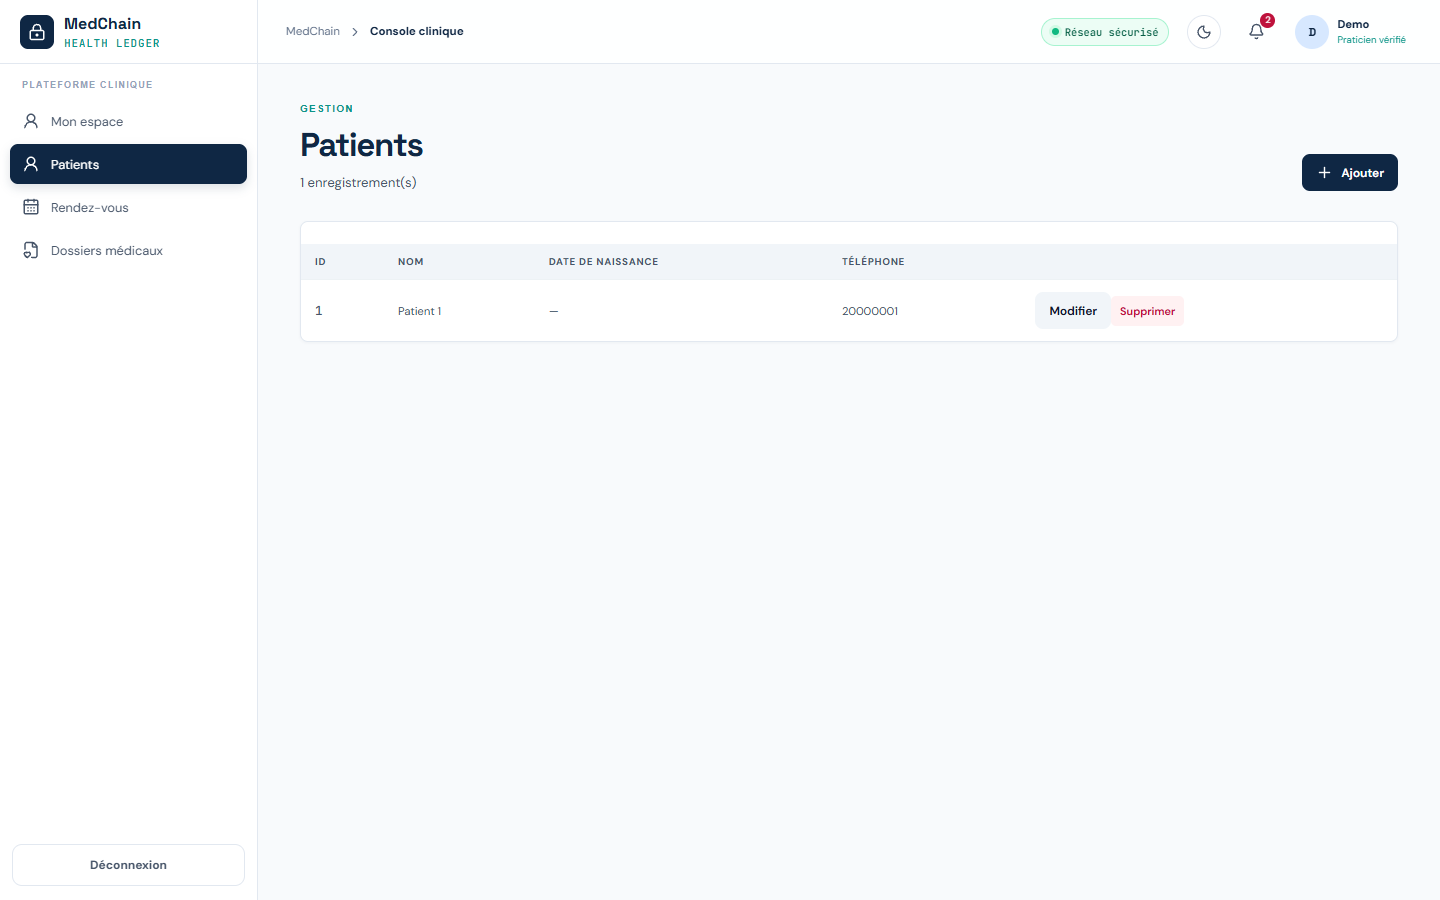
\includegraphics[width=\textwidth]{S12-liste-patients.png}
\caption{Liste des patients}
\label{fig:patients_list}
\end{figure}

\begin{figure}[H]
\centering
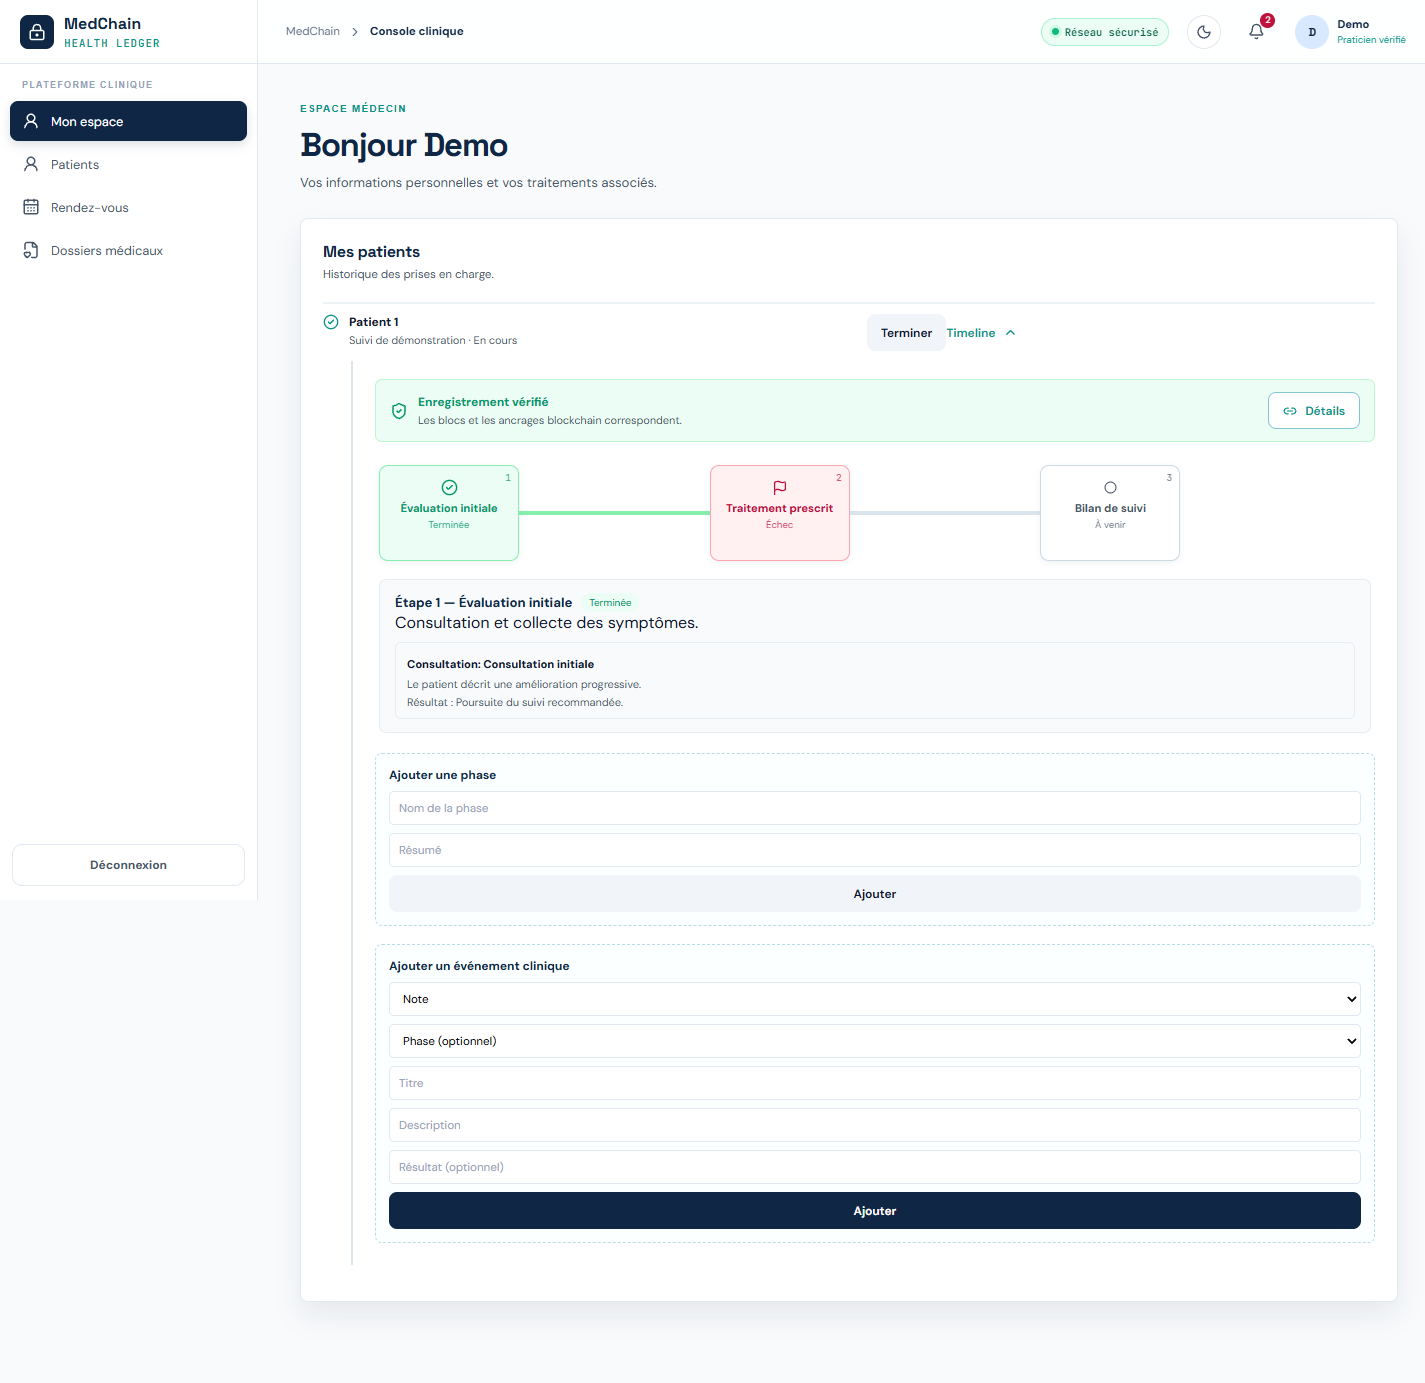
\includegraphics[width=\textwidth]{S13-ajout-evenement-traitement.png}
\caption{Timeline et ajout d'un événement clinique}
\label{fig:event_form}
\end{figure}

\section{Conclusion}

Le parcours de soins est désormais couvert de bout en bout, avec une visualisation de l'état d'intégrité directement dans l'interface. Le chapitre suivant décrit le chiffrement, la formation des blocs et l'ancrage.
